% Draft 1 of sections 2 to 4, written on 2026-11-05 on the PI's word (log.md 0066).
% Body text only, for the JGAA LaTeX package, which is not yet in the repository. Every number traces to the record named in the comment beside it.
% Citation keys are placeholders, listed in refs-todo.md, and no bibliographic detail has been filled in from memory.

\section{Problem and Model}
\label{sec:model}

\paragraph{Graphs and Streams.}
A stream is a sequence of events $(t, u, v, \sigma)$ with a timestamp $t$, two vertices and an operation $\sigma$ that inserts or deletes the undirected edge $\{u, v\}$.
Self-loops are dropped, direction is dropped, and the graph is kept under set semantics: inserting a present edge or deleting an absent one changes nothing.
This is the cleaning of Hanauer et al.~\cite{hanauer-dyncount}, whose instance set our streams come from (Section~\ref{sec:streams}).
Every stream starts from the empty graph.
% gate0-protocol.md, Stream construction; m1d07-streams.md, cleaning rule

\paragraph{Three Labels.}
Each stream carries one of three labels, and every table states it.
\emph{Real timestamps, insert-only}: the events of a temporal file in time order, with no deletion.
\emph{Real timestamps, synthetic expiry}: the same insertions, each followed by the deletion of its edge fourteen days later, with deletions before insertions at equal times, as in Hanauer et al.~\cite{hanauer-dyncount} after Chen et al.~\cite{chen-expiry}.
\emph{Real timestamps, real deletions}: the link streams of six Wikipedia editions from KONECT~\cite{konect,preusse-wiki}, whose deletions are recorded events, in which 16\% to 28\% of the events are deletions.
No fully synthetic stream enters any result.
% CLAUDE.md hard rule 4; gate0-protocol.md; m1d07-streams.md; outline.md readiness test 5

\paragraph{Batches.}
A stream is cut into consecutive batches of $c$ events, with $c = 100$ and $c = 1{,}000$.
A batch is first reduced to its net effect: an edge whose state at the end of the batch equals its state at the start is dropped, and every other edge becomes one net insertion or one net deletion.
After each batch an algorithm reports the exact number of copies of $C_p$, the cycle on $p$ vertices, in the current graph, for $p \in \{3, 4, 5\}$.
An answer that differs from the true count on any batch is a failure, whatever its time.
% gate1-protocol.md, Streams; CLAUDE.md hard rule 1

\paragraph{The Delta of One Update.}
All algorithms in this paper apply the net updates of a batch one at a time and add up their deltas.
For an update of the pair $\{u, v\}$, the delta is $\pm$ the number of $p$-cycles that the pair closes, counted in the graph without the pair, that is, before the insertion or after the deletion.
Writing $N(x)$ for the neighbourhood of $x$ in that graph, $d(x) = |N(x)|$ for its degree, and $W[a, b] = |N(a) \cap N(b)|$ for the number of common neighbours,
\begin{align*}
  \Delta_3(u, v) &= W[u, v], \\
  \Delta_4(u, v) &= \sum_{a \in N(u)} W[a, v], \\
  \Delta_5(u, v) &= \sum_{b \notin \{u, v\}} A[b]\, C[b] \;-\; \sum_{t \in N(u) \cap N(v)} \bigl(d(t) - 2\bigr),
\end{align*}
where $A[b]$ counts the paths $(u, a, b)$ with $a \neq v$, and $C[b]$ the paths $(v, c, b)$ with $c \neq u$.
The sum $\sum_b A[b] C[b]$ counts every triple $(a, b, c)$, and the only triples that do not form a path $(u, a, b, c, v)$ on five distinct vertices are those with $a = c$.
Such a vertex $t = a = c$ lies in $N(u) \cap N(v)$, and each of its neighbours other than $u$ and $v$ gives one such triple, which is the second term.
Applying the updates in sequence counts every cycle created or destroyed by the batch exactly once, because the deltas telescope.
This is the delta-query rule of Ammar et al.~\cite{ammar-delta} with one update per step, and we do not claim it.
% benchmarks/gate1.cpp header, COMMON TO ALL; benchmarks/fivecycle.cpp header, THE FORMULA; CLAUDE.md hard rule 6

\paragraph{All Costs Count.}
The time of a batch includes reducing the batch to its net updates, grouping it where an algorithm groups, updating the graph, and maintaining every auxiliary structure: wedge tables, lists of heavy vertices, and the switch of a vertex between heavy and light.
No structure is built ahead of the stream, and no algorithm reads beyond the current batch.
% CLAUDE.md hard rules 5 and 7

\section{Kernels}
\label{sec:kernels}

Table~\ref{tab:arms} lists the kernels, which we also call arms.
Each arm computes the deltas of Section~\ref{sec:model} in its own way, and all arms of a pattern give the same count after every batch.

\begin{table}[t]
  \centering
  \begin{tabular}{lccc}
    \hline
    Role & $p = 3$ & $p = 4$ & $p = 5$ \\
    \hline
    Per-update scan & S3 & S4 & R2 \\
    \textbf{Sharing, star row} & \textbf{P3} & \textbf{P4} & \textbf{PR} \\
    Wedge table, tuned layout & T3 & T4 & WT \\
    Wedge table, flat & & & WJ \\
    Mixed table, hubs scanned & M3 & M4 & M5 \\
    Affected-subgraph recount & & A4 & A5 \\
    Published batch sharing, port & & B4 & \\
    \hline
  \end{tabular}
  \caption{The arms. Sharing arms in bold.}
  \label{tab:arms}
\end{table}
% gate1-protocol.md, Arms

\paragraph{Scan.}
S3, S4 and R2 compute each delta from the adjacency lists alone.
R2, at $p = 5$, builds the row $A$ at the endpoint of lower degree and streams the other side through it, so that $\sum_b A[b] C[b]$ is read without storing $C$.
% fivecycle.cpp, FORMS, R2

\paragraph{Sharing by Star Rows.}
A batch's net updates often share an endpoint: a user who posts several answers in one batch adds several edges at one vertex.
The sharing arms group the net updates of a batch into stars.
Each update goes to the endpoint at which the batch has more updates, its pivot, and the updates at one pivot $x$ form a star whose spokes are the other endpoints.
For a star at $x$, PR builds the row $A$ at $x$ once and adjusts it by each spoke in turn, so that each spoke sees the graph with the earlier spokes already applied.
Each spoke then streams its own side through the shared row, as R2 does.
For a star with one spoke PR runs R2 itself, so PR can lose to R2 only by the cost of grouping.
Figure~\ref{fig:workedbatch} shows one batch of a real stream: its largest star has 24 spokes, and the shared row costs 6,097 operations where one row per spoke costs 64,445.

\begin{figure}[tbp]
  \centering
  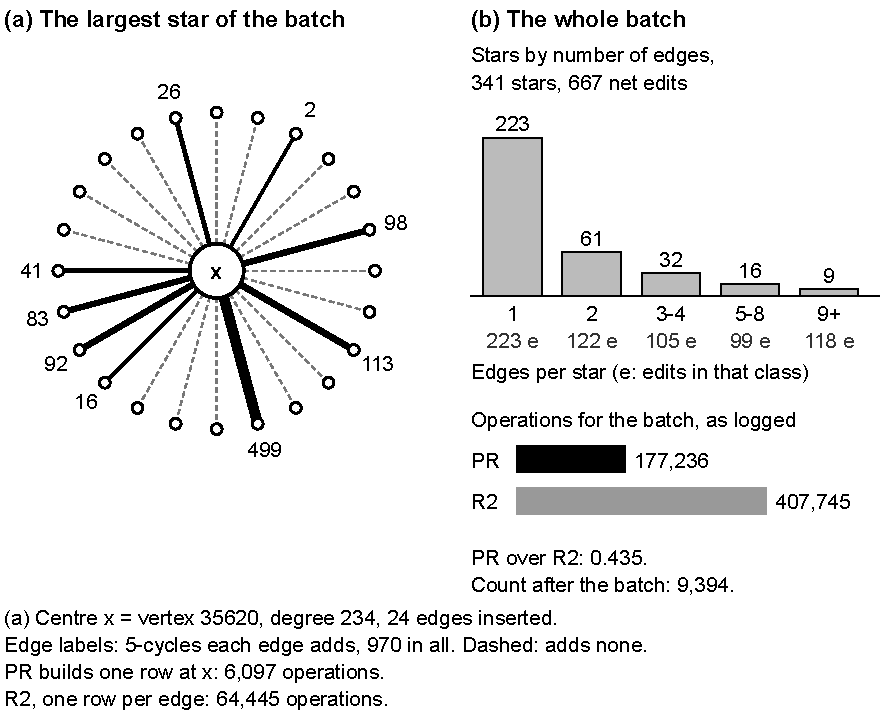
\includegraphics[width=\textwidth]{fig-worked-batch}
  \caption{A worked batch: batch 465 of the 1,454 batches of sx-askubuntu with synthetic expiry, at 1,000 events per batch and $p = 5$. The 1,000 events net to 667 edits. Panel (a) shows the largest star of the batch, 24 insertions at one vertex, each edge labelled with the 5-cycles it adds: PR builds one row at the centre for 6,097 operations, where R2 builds one row per edge for 64,445. Panel (b) shows the whole batch: its 341 stars by number of edges, and the operations of PR and R2, 177,236 against 407,745. The batch was chosen by a rule fixed before any batch was read: the median of PR over R2 among the batches where PR does fewer operations. Operation counts from the count build, not time: on the clock, PR over R2 on this cell is 0.588, a smaller gain than the 0.435 in operations.}
  \label{fig:workedbatch}
\end{figure}
P3 and P4 apply the same idea to triangles and 4-cycles.
They carry a guard that reads only degrees, has no tuned parameter, and whose own operations are counted: a star keeps its row only if the row costs less than the scans it replaces, and otherwise its spokes run as S3 or S4.
The guard is needed because S4 walks from the endpoint of lower degree, while a row is always built at the centre. In early tests, a star at a hub with a few small spokes made P4 slower than S4.
PR has no guard. A guard could only make PR faster, so leaving it out can only understate the gain of sharing.
Reusing one row per vertex across a batch is published for triangle listing by DPTL+~\cite{dptl} and for butterfly counting by BFCB-IG~\cite{bfcb}, and grouping a batch into stars for general patterns by Cheetah~\cite{cheetah}, together with the finding that triangles gain least. We do not claim either.
% gate1.cpp, guards; fivecycle.cpp, FORMS, PR; gate1-protocol.md, Arms; log.md 0019

\paragraph{Wedge Tables.}
T3, T4, WT and WJ keep $W[a, b]$ for every pair of vertices with a common neighbour, and update it on every edge edit.
A delta then becomes a sum of table reads: $W[u, v]$ at $p = 3$, a sum over $N(u)$ at $p = 4$, and at $p = 5$
\[
  \Delta_5(u, v) = \sum_{\substack{a \in N(u),\ c \in N(v) \\ a \neq c}} W[a, c] \;-\; \tau\,(d(u) - 1) \;-\; \tau\,(d(v) - 1),
  \qquad \tau = |N(u) \cap N(v)|,
\]
with $W$ taken in the graph without the pair.
WJ stores the table in one flat hash map.
WT holds the same entries in one open-addressing table per vertex, with each pair stored in both of its tables, so that a join reads only the tables of the shorter list.
Its slots are four bytes, they are searched four at a time with SSE2, and the join switches from probes to one pass over the table against a bitset when that is cheaper.
The layout of WT was chosen by trial on synthetic R-MAT streams~\cite{rmat}, so no stream of this paper shaped it.
T3 and T4 use WT's table.
% fivecycle.cpp, WT and FORMS, WJ; gate1.cpp, T

\paragraph{Mixed Tables.}
M3, M4 and M5 follow the idea of Hanauer, Henzinger and Hua~\cite{hhh}: the table holds only the wedges through light centres, so a hub pays no upkeep, and the wedges through hubs are counted from the adjacency lists at query time.
A vertex turns heavy above degree $2\theta$ and light again below $\theta$, so a switch costs at most $(2\theta)^2$ pairs and is paid for by at least $\theta$ updates.
Writing $H$ for the set of heavy vertices, the hub term at $p = 5$ is $\sum_{h \in H} (A[h] C[h] - T[h])$, with $A[h] = |N(u) \cap N(h)|$, $C[h] = |N(v) \cap N(h)|$ and $T[h] = |N(u) \cap N(v) \cap N(h)|$.
One value of the threshold $\theta$ per pattern was chosen on the engineering streams of Section~\ref{sec:method}, before any evaluation run of a mixed table, from $\{16, 32, \dots, 1024\}$: 16 at $p = 3$ and $p = 4$, and 128 at $p = 5$.
Section~\ref{sec:sensitivity} gives M5 its best $\theta$ per cell instead.
% gate1.cpp, M; gate1-protocol.md, Theta; results/gate1-M1D04/theta.txt; M1D06A

\paragraph{Recount and Published Sharing.}
A4 and A5 recount the cycles inside the ball of radius $r$ around each changed edge, $r = 1$ at $p = 4$ and $r = 2$ at $p = 5$, in the union of the old and new graphs, and take the difference.
The static counters are Chiba and Nishizeki's wedge pairing~\cite{chiba-nishizeki} at $p = 4$ and Algorithm~1 of Shi, Huang and Shun~\cite{shi-huang-shun} at $p = 5$.
B4 ports the batch 4-cycle algorithm BFCB-IG of Wang et al.~\cite{bfcb} from bipartite to general graphs.
It splits a mixed batch into deletions and then insertions, as BFCB-IG does, and builds one row per start vertex that every edit at that vertex reads.
We know of no batch algorithm of this form for 5-cycles, so B4 has no counterpart at $p = 5$.
There is no recount at $p = 3$: in an earlier operation count of ours on six of the streams of Section~\ref{sec:method}, a triangle update cost 5.9 to 13.9 operations, and a recount cannot compete with that.
% gate1.cpp, A and B4; gate1-protocol.md, Arms

\paragraph{Exactness.}
An oracle test compares every arm of every pattern with a brute-force count over vertex tuples, after every batch, on random small graphs whose batches hold deletions, hubs, whole stars, repeated pairs and no-op edits.
Mixed arms run there at $\theta$ down to 1, so vertices switch on graphs this small.
Fourteen mutants, each a plausible way to get an arm wrong, must each fail the test, and so must a naive per-edge sum, which counts a cycle once for each of its changed edges.
On the streams, every arm's count matches every other arm's after every batch, in every timing repeat and in every count build.
% tests/test_gate1.cpp header; CLAUDE.md hard rules 1 and 2; results/gate1-M1D04/README.md

\section{Method of Measurement}
\label{sec:method}

\paragraph{Streams and Their Roles.}
\label{sec:streams}
Twenty streams enter the study, in four sets that were fixed before any of them was timed.
The \emph{engineering} streams, CollegeMsg~\cite{panzarasa-collegemsg}, email-Eu-core-temporal and sx-mathoverflow~\cite{paranjape-motifs}, were used to choose $\theta$ and to fit the cost model of Section~\ref{sec:costmodel}, and never enter a verdict.
The \emph{evaluation} streams, sx-askubuntu, sx-superuser and wiki-talk-temporal~\cite{paranjape-motifs,leskovec-wiki-governance}, decide the first verdict.
These six streams and sx-stackoverflow come from SNAP~\cite{snap}.
The \emph{held-out} stream, sx-stackoverflow, was chosen before any timing run and timed once, at $p = 5$ only.
Hanauer et al.'s set~\cite{hanauer-dyncount} has 56 instances, 18 of them real streams, and four of those 18 are in the first three sets. The \emph{new} streams are 13 of the other 14, chosen by a rule written before their sizes were read: six Wikipedia link streams with real deletions from KONECT, two Reddit hyperlink streams from SNAP~\cite{kumar-reddit}, and five temporal files from Network Repository~\cite{network-repository}.
Each is cut to its first 2,000,000 events, which is Hanauer et al.'s own prefix.
One of them, soc-youtube-growth, has a single timestamp in that prefix and is reported but never scored.
The 38 Kronecker streams of Hanauer et al.'s set are left out as fully synthetic.
Expiry and insert-only variants run on every stream without real deletions, at both batch sizes.
We call one combination of a stream, its variant, a batch size and a pattern size a \emph{cell}.
% gate1-protocol.md, Streams; m1d07-streams.md; docs/figures/fig-test-set.svg; log.md 0025

\paragraph{Operations First.}
Each arm exists in two builds from one source.
The count build counts every unit operation: a list element scanned, a lookup of an edge in the graph's hash map, a row read or write, a table read or write, a degree read, a graph edit, and each step of reducing and grouping the batch.
Operation counts are deterministic and do not depend on the machine, and they were read before any clock.
The timing build has no counters, because a counter in a hot loop is a store the compiler cannot move, and on a synthetic stream the counters cost R2 and PR about 15\% and WJ about 1\%.
All seconds in this paper come from the timing build, and all operation counts from the count build.
Figure~\ref{fig:timeline} shows the count and the operations of five kernels over a whole stream.

\begin{figure}[tbp]
  \centering
  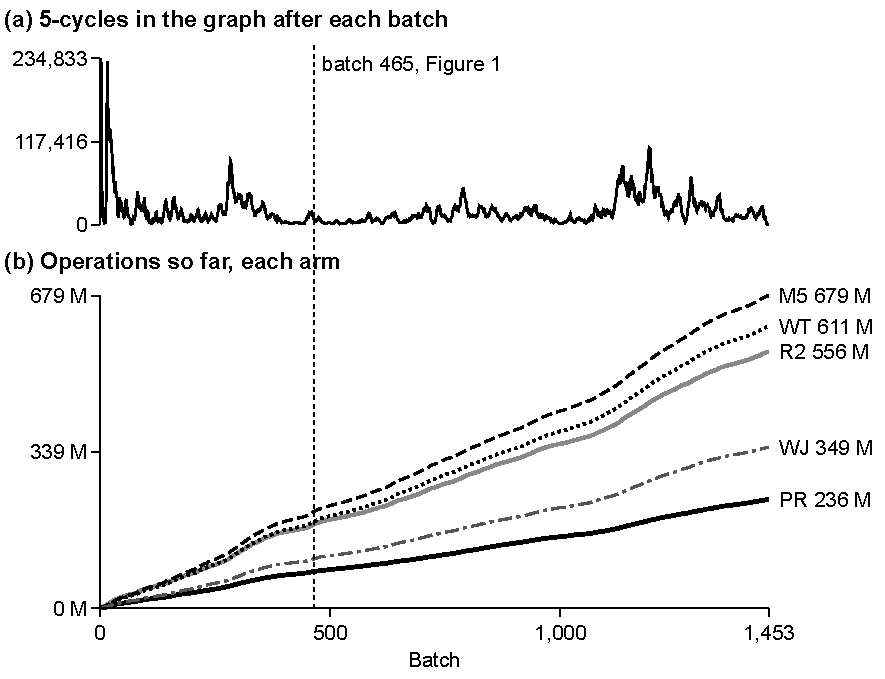
\includegraphics[width=\textwidth]{fig-stream-timeline}
  \caption{The same stream over all 1,454 batches: (a) the 5-cycle count after each batch, and (b) the cumulative operations of PR, R2, WT, WJ and M5. Every kernel's count agrees on every batch. The expiry rule empties the graph by the end of the stream. Operation counts from the count build, not time. On this cell PR also does the fewest operations; on the insert-only cells of the sx streams WJ does fewer operations than PR and is slower, so this cell is not the general case.}
  \label{fig:timeline}
\end{figure}
% fivecycle.cpp header; CLAUDE.md hard rule 3

\paragraph{The Clock.}
All runs are on one machine, an Intel Core Ultra 7 265 with 31\,GB of memory and a 30\,MB last-level cache, under Windows 11, with GCC 16.2 at \texttt{-O2}, linked statically.
One process runs at a time, pinned to one performance core, logical CPU 8.
On a cell whose fastest arm takes under 60\,s each arm runs five times, and otherwise three, with the arms interleaved across repeats in a rotated order.
An arm more than five times slower than the fastest on a cell runs once.
A process stops at 1,200\,s or 16\,GB of committed memory, and A4 and A5 stop at 300\,s.
An arm stopped by time has not finished. It is never counted as a win, and in comparisons its time is its limit.
An arm stopped by memory is out of that cell.
% gate1-protocol.md, Measure; STATUS.md, Environment

\paragraph{The Rule, Fixed Before the Clock.}
Let \emph{share} be P3, P4 or PR, or at $p = 4$ the faster of P4 and B4. Let \emph{best} be the fastest of the other arms, leaving out B4. An arm stopped by its time limit counts in this comparison with its time set to the limit.
A cell \emph{passes} when the slowest repeat of share is at most $0.67$ times the fastest repeat of best.
Comparing the slowest repeat with the fastest is deliberate. In an earlier experiment of ours, a cell passed when the fastest repeats were compared, by a difference of one clock tick, and failed when the slowest of three repeats was used.
A cell's \emph{score} is the ratio of the medians. A cell is \emph{scored} if share and at least one other arm finished or were stopped by time.
The verdict at $p = 5$ is Go if at least a third of the scored cells pass, on at least two streams, with at least two expiry cells among them.
These thresholds, and the treatment of stopped arms, were fixed before the first timing run and were not changed after it.
% gate1-protocol.md, Rule; log.md 0025, reading M1D04-R1

\paragraph{What Exclusive Means.}
The machine is shared with other projects, and timing ran only while it was reserved for this study: no other long or parallel process ran during a timing run.
The machine was not silent.
Scheduled tasks of another project ran every quarter hour, a status mail ran every two hours, and desktop sessions stayed open.
After each timing run, every timed process was checked against the recorded start times of these tasks, and repeats that overlapped one were compared with clean repeats of the same arm on the same cell.
In the last timing run, for the cost model, one of 790 scored repeats overlapped a known task, and it ran 0.2\% over its arm's median.
Section~\ref{sec:sensitivity} gives the same comparison for the runs on the new streams.
% log.md 0025, 0036, 0065; scripts/overlap_check.py; results/cost-M1D10/README.md

\paragraph{Cores.}
To test whether a verdict depends on the core, the 24 cells nearest the pass line were timed again on a performance core and on an efficiency core of the same processor, in one timing run.
The two kinds of core differ in design and in their first two cache levels, and share the last-level cache and memory.
So this is not a second machine, and the paper does not use it as one.
% docs/experiments/m1d08-core-type.md; results/gate1-M1D08/README.md
